\documentclass[12pt,letterpaper]{article}
\usepackage{apa_manual}
\apatituloCorto{Validación causal e inferencia estadística}

\begin{document}

\apacabecera
  {Validación causal, pruebas pareadas, experimento sintético e inferencia múltiple}
  {Manual teórico y práctico 7 — Fundamento completo de las Etapas 5, 6, 7 y 8}
  {En series de revisiones es muy fácil cometer errores silenciosos que inflan artificialmente los resultados, como usar rezagos cuya revisión todavía no concluye o realizar decenas de contrastes sin corregir por multiplicidad. Este manual explica la regla estricta de causalidad en tiempo real, las pruebas de comparación de pronósticos, las simulaciones Monte Carlo y cálculo de potencia de la Etapa~6, la inferencia integrada de la Etapa~8 y la regla de paro que cerró la Etapa~7.}

\section{La regla de oro para no mirar el futuro en revisiones (Etapa 5)}

Supongamos que estamos parados en junio de 2020 (\(v_0 = \texttt{2020-06}\)), cuando acaba de publicarse por primera vez el desplome de abril de 2020 (\texttt{2020m4}), y deseamos pronosticar cuánto terminará corrigiéndose once meses después. Aunque enero o febrero de 2020 ya sucedieron en el calendario, sus revisiones acumuladas a \(H = 11\) meses \emph{todavía no existen en junio de 2020}, porque sus publicaciones finales \(v_{11}\) recién aparecerán en 2021. Entrenar un modelo con observaciones cuya ventana \(v_{11}\) cierra después de \(v_0(t)\) violaría la flecha del tiempo.

Por esta razón, la función \codigo{get\_causal\_train\_indices} en \codigo{scripts/rtd\_eval\_utils.py} impone la condición estricta de causalidad para todo período candidato de entrenamiento \(s < t\):
\begin{equation}
  v_{11}(s) \le v_0(t).
  \label{eq:regla_causal}
\end{equation}
La Figura~\ref{fig:linea_causal} muestra esta frontera temporal sobre un ejemplo real. Como el rezago de primera publicación es \(v_0(t) \approx t + 2\) meses y el cierre a horizonte \(11\) ocurre en \(v_{11}(s) \approx s + 13\) meses, la Ecuación~\ref{eq:regla_causal} exige \(s + 13 \le t + 2\), es decir, \(t - s \ge 11\). Ese es exactamente el motivo por el cual el primer rezago completado utilizable es \codigo{Y\_lag11}, quedando estrictamente prohibidos \(Y_{t-1}, \dots, Y_{t-10}\).

\begin{figure}[htbp]
  \caption{Línea temporal causal que impide entrenar con revisiones aún incompletas en \(v_0(t)\)}
  \label{fig:linea_causal}
  \centering
  \begin{tikzpicture}[font=\scriptsize, >=Stealth]
    \draw[->, thick, apaSlate] (0,0) -- (13.2,0) node[right] {Calendario};
    \foreach \x/\lbl in {0.8/2019m3, 3.3/2019m5, 5.8/2020m2, 8.3/2020m4, 10.6/2020m6, 12.6/2021m5} {
      \draw (\x,0.12) -- (\x,-0.12);
      \node[below=2pt] at (\x,-0.12) {\lbl};
    }

    \draw[|-|, very thick, apaGreen] (3.3, 1.38) -- (8.3, 1.38)
      node[midway, above=2pt, align=center] {Ventana completada de \codigo{2019m3}:\\ \(v_0=\text{2019m5} \longrightarrow v_{11}=\text{2020m4} \le v_0(t)\;\checkmark\)};

    \draw[|-|, very thick, apaAccent, dashed] (8.3, 0.72) -- (12.6, 0.72);
    \node[above=2pt, fill=white, inner sep=1.5pt, text=apaAccent, align=center] at (7.45, 0.80)
      {Ventana incompleta de \texttt{2020m2}: \(v_{11}\) cierra en 2021 \(\times\)};

    \draw[very thick, apaNavy] (10.6, 0.0) -- (10.6, 2.28)
      node[above, align=center, font=\scriptsize\bfseries] {Fecha real de pronóstico\\ \(v_0(\texttt{2020m4}) = \texttt{2020-06}\)};
    \fill[apaNavy] (10.6, 0.0) circle (2.2pt);
  \end{tikzpicture}
  \apanota{Implementación verificada en \codigo{scripts/rtd\_eval\_utils.py} (\texttt{df["v\_H11\_date"] <= v0\_now}).}
\end{figure}

Adicionalmente, toda imputación de faltantes por mediana, estandarización (\(z\)-score), extracción de factores PCA y selección interna de hiperparámetros se ajusta únicamente sobre \codigo{tr\_idx} antes de predecir el origen \(t\). Al final de la muestra se reserva el bloque congelado de \(n = 60\) meses (\texttt{2019m12}--\texttt{2024m11}) para evitar selección adaptativa ex post, y una prueba automatizada de corrupción de datos futuros (Etapa~4) confirma una diferencia máxima exactamente igual a \(0{,}0\) al alterar todos los valores posteriores a \(v_0(t)\).

\section{Métricas de evaluación y pruebas estadísticas pareadas}

Sobre la secuencia de \(N = 250\) errores fuera de muestra \(e_t = Y_t^{(11)} - \widehat{Y}_t\), evaluamos principalmente la raíz del error cuadrático medio (RMSE), el error absoluto medio (MAE) y el \(R^2\) fuera de muestra respecto al promedio del bloque evaluado:
\begin{equation}
  \text{RMSE} = \sqrt{\frac{1}{N}\sum_{t=1}^{N} e_t^2}, \qquad \text{MAE} = \frac{1}{N}\sum_{t=1}^{N} \lvert e_t \rvert, \qquad R^2_{\text{OOS}} = 1 - \frac{\sum_{t=1}^{N}(Y_t - \widehat{Y}_t)^2}{\sum_{t=1}^{N}(Y_t - \bar{Y}_{\text{OOS}})^2}.
  \label{eq:rmse_r2}
\end{equation}
Descartamos expresamente el MAPE porque el denominador \(Y_t^{(11)}\) toma el valor exacto \(0{,}0\) con alta frecuencia (percentil~25 igual a cero), volviendo inestable cualquier porcentaje relativo.

Cuando dos modelos exhiben RMSE distintos, debemos verificar mediante tres herramientas implementadas en \codigo{rtd\_eval\_utils.py} si la diferencia es estadísticamente real:
\begin{enumerate}
  \item \textbf{Diebold--Mariano con ajuste Harvey--Leybourne--Newbold \parencite{diebold1995, harvey1997}:} define el diferencial de pérdida \(d_t = L(e_{t,\text{modelo}}) - L(e_{t,\text{bench}})\), bajo pérdida cuadrática \(e_t^2\) o absoluta \(\lvert e_t \rvert\). Valores \(\bar{d} < 0\) favorecen al modelo evaluado. Dividimos \(\bar{d}\) por su error estándar Newey--West usando ancho de banda \(L_{\text{uso}} = \max(L_{\text{NW}}, \min(H, \lfloor N/4\rfloor))\), aplicamos el factor corrector de muestra finita \(\sqrt{\frac{N + 1 - 2h + h(h-1)/N}{N}}\) y evaluamos el \(p\)-valor bilateral bajo una distribución \(t_{N-1}\).
  \item \textbf{Clark--West para modelos anidados \parencite{clark2007}:} cuando un modelo grande contiene a otro pequeño más variables adicionales, el modelo grande asume varianza de estimación extra aunque los nuevos coeficientes verdaderos sean nulos. Clark--West ajusta esa penalización mediante:
  \begin{equation}
    f_t = e_{t,\text{pequeño}}^2 - \left[ e_{t,\text{grande}}^2 - (\widehat{Y}_{t,\text{pequeño}} - \widehat{Y}_{t,\text{grande}})^2 \right].
    \label{eq:clark_west}
  \end{equation}
  \emph{Lección de cautela en Perú:} durante choques extremos como abril de 2021, si el modelo grande extrapola mal (\codigo{Ridge} predijo \(+4{,}020\) p.p.), el término \((\widehat{Y}_{\text{media}} - \widehat{Y}_{\text{Ridge}})^2\) crece desmesuradamente e infla el estadístico CW (\(3{,}554\), \(p=0{,}00019\)) aunque el RMSE crudo haya empeorado. Por ello nunca debe leerse CW de forma aislada sin revisar la trayectoria acumulada de pérdida cuadrada (Figura~\ref{fig:cum_se}).
  \item \textbf{Bootstrap circular por bloques \parencite{politis1992}:} reordenar meses individuales al azar destruiría la dependencia de \(11\) meses de solapamiento y el ciclo anual. Por eso sorteamos \(B = 2\,000\) remuestras uniendo bloques continuos de \(L = 12\) meses (envolviendo circularmente el final de la serie con el inicio) para construir intervalos de confianza al \(95\%\) de \(\text{RMSE}_{\text{modelo}} - \text{RMSE}_{\text{bench}}\).
\end{enumerate}

\begin{figure}[htbp]
  \caption{Trayectoria de pronósticos y pérdida cuadrada acumulada relativa frente a Ridge (Etapa~3)}
  \label{fig:cum_se}
  \centering
  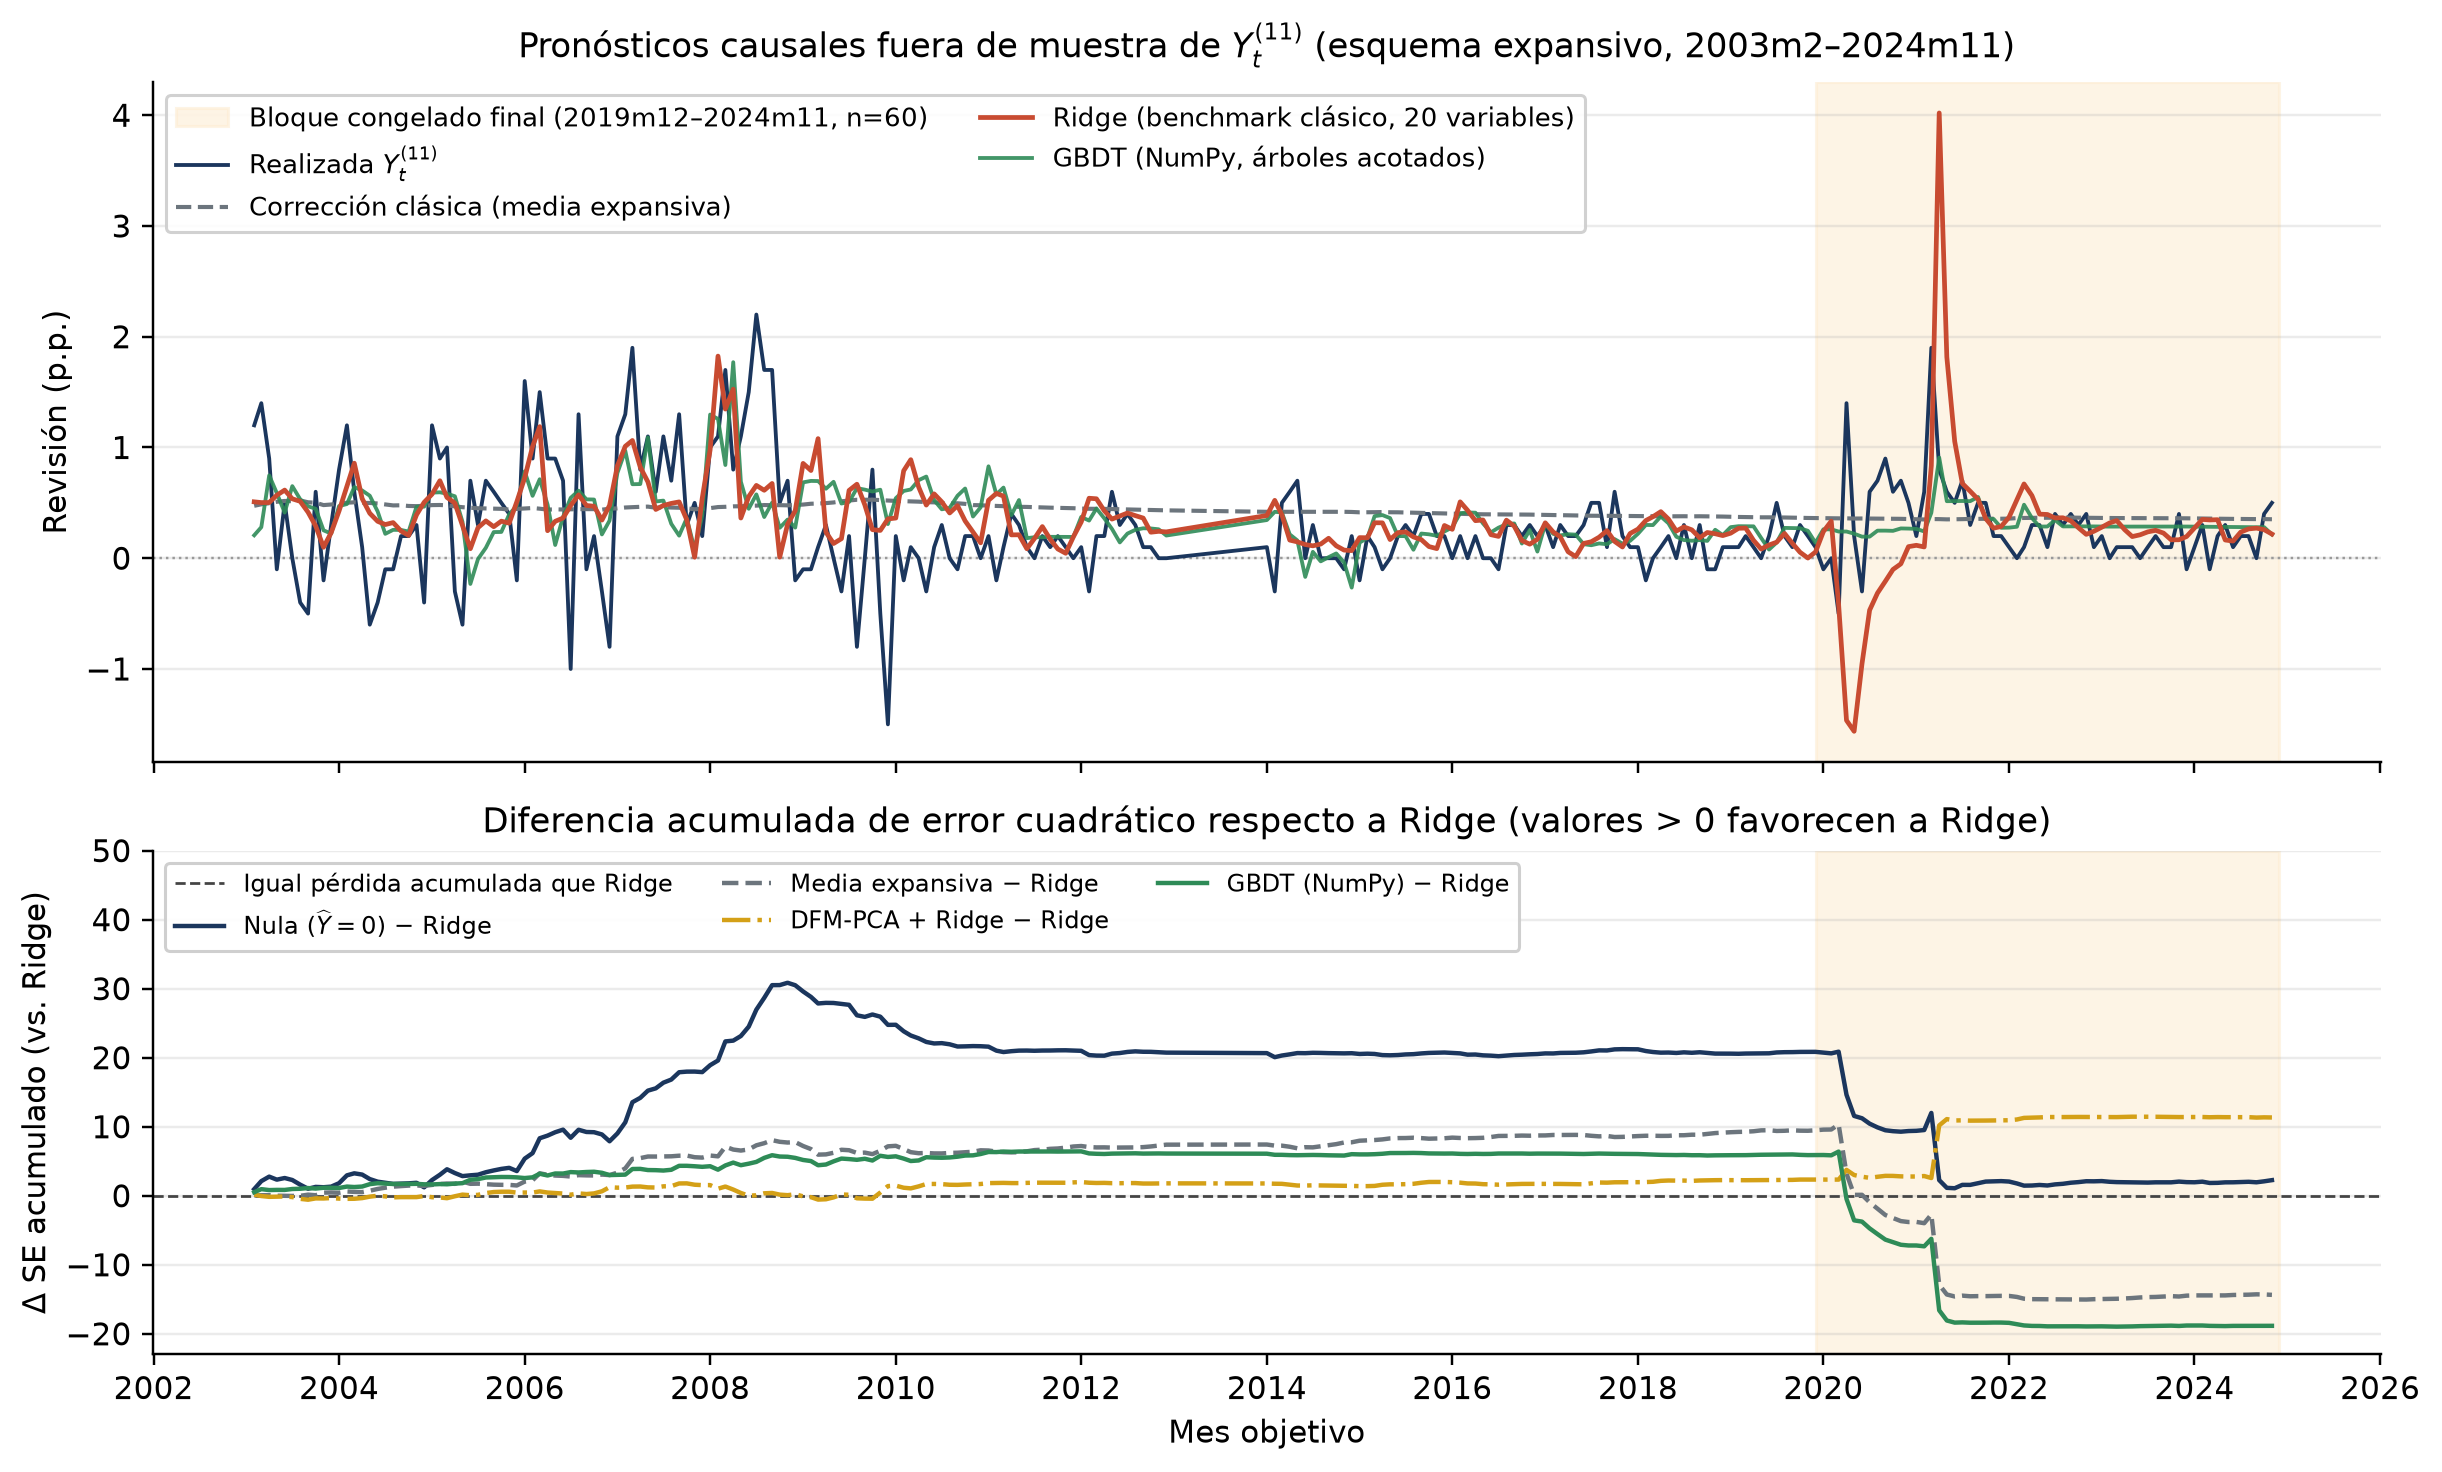
\includegraphics[width=0.93\textwidth]{figuras/etapa3_oos_predicciones.png}
  \apanota{Tomado de \codigo{output/etapa3\_clasicos/etapa3\_oos\_predicciones.png}. Una curva ascendente indica ventaja de \codigo{Ridge}; la caída vertical en 2020--2021 muestra el impacto puntual del choque COVID.}
\end{figure}

\section{Multiplicidad, Model Confidence Set y regla de cierre (Etapas 7 y 8)}

Cuando comparamos \codigo{QRC\_Ising5} contra siete competidores simultáneamente (\codigo{Zero}, \codigo{BiasCorr\_Mean}, \codigo{AR\_BIC}, \codigo{Ridge}, \codigo{GBDT\_NumPy}, \codigo{ESN\_20} y \codigo{RFF\_20}), realizar siete pruebas independientes a nivel \(\alpha = 0{,}05\) eleva la probabilidad de obtener al menos un falso positivo por puro azar hasta \(1 - (1 - 0{,}05)^7 \approx 30{,}2\%\). La Etapa~8 (\codigo{scripts/etapa8\_inferencia\_y\_cierre.py}) controla este riesgo mediante tres pilares formales:
\begin{itemize}
  \item \textbf{Holm--Bonferroni \parencite{holm1979}:} ordena los \(m = 7\) valores \(p_{(1)} \le \dots \le p_{(m)}\) y multiplica cada uno por \((m - k + 1)\) imponiendo monotonicidad creciente, controlando estrictamente la tasa de error por familia (FWER).
  \item \textbf{Benjamini--Hochberg \parencite{benjamini1995}:} escala cada \(p_{(k)}\) por \(m / k\) imponiendo monotonicidad decreciente para controlar la tasa de falsos descubrimientos (FDR) como complemento menos conservador.
  \item \textbf{Model Confidence Set de \textcite{hansen2011}:} evalúa conjuntamente a los \(12\) modelos sin privilegiar un único referente. Mediante el estadístico \(T_{\max}\) y bootstrap circular compartido (\(B=2\,000\), \(L=12\)), elimina iterativamente al modelo con mayor pérdida relativa estandarizada \(t_i = \bar{d}_{i\cdot}/\hat{\sigma}_{i\cdot}\) hasta que no puede rechazarse la igualdad entre los sobrevivientes; todo modelo con \(p_{\text{MCS}} \ge 0{,}10\) pertenece al conjunto \(\text{MCS}_{90\%}\) (y a \(\text{MCS}_{75\%}\) si \(p_{\text{MCS}} \ge 0{,}25\)).
\end{itemize}

\begin{figure}[htbp]
  \caption{Supervivencia en el Model Confidence Set y familia confirmatoria Holm--Bonferroni (Etapa~8)}
  \label{fig:etapa8_mcs}
  \centering
  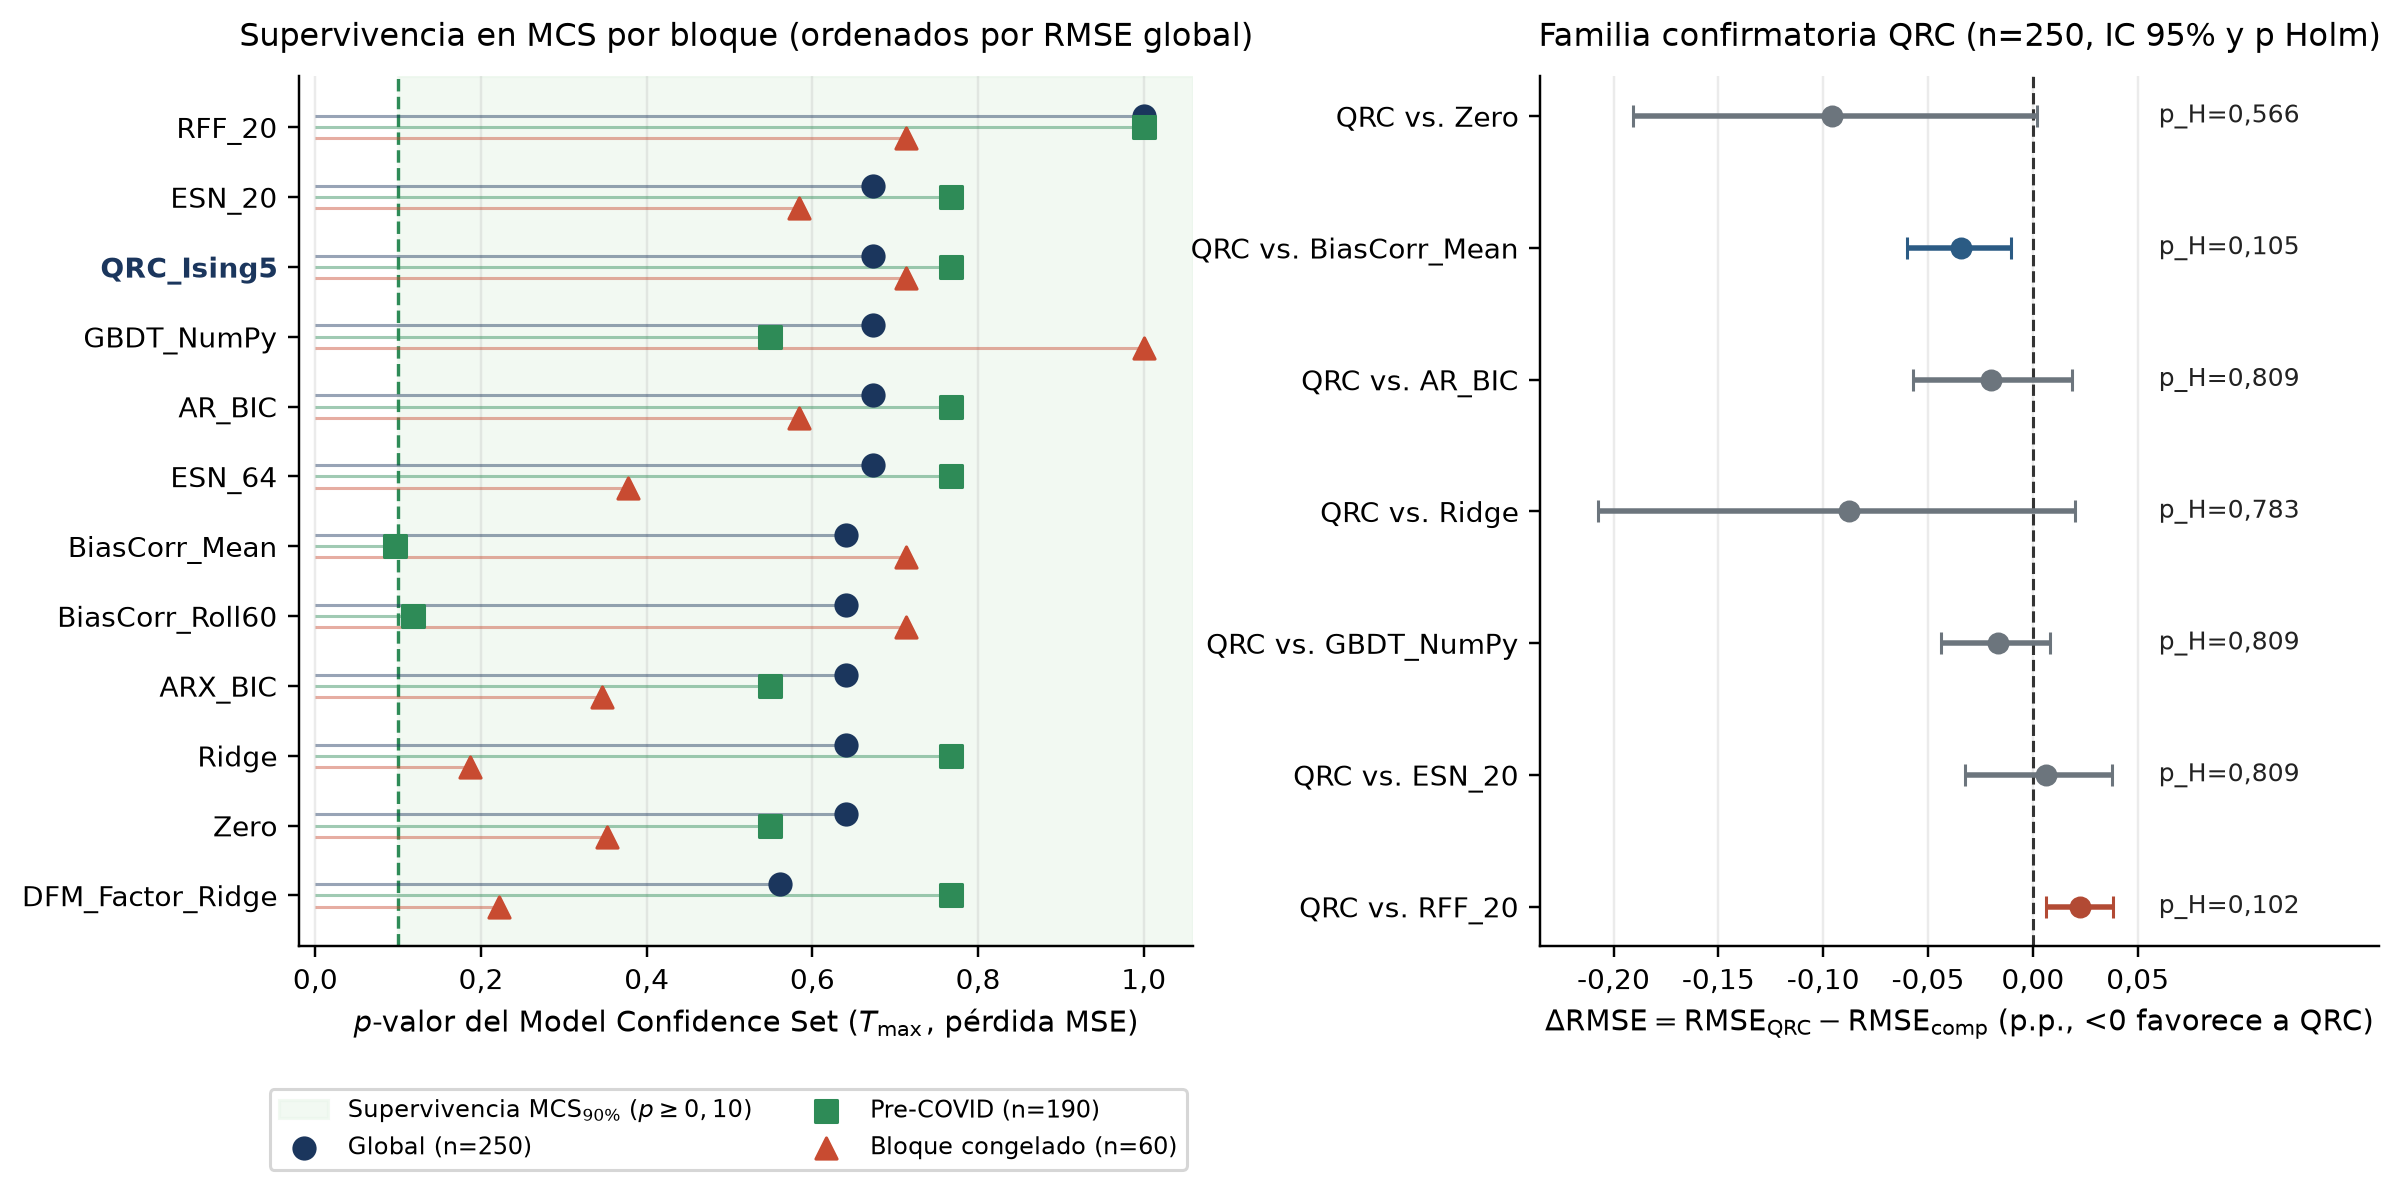
\includegraphics[width=0.95\textwidth]{figuras/etapa8_mcs_inferencia.png}
  \apanota{Tomado de \codigo{output/etapa8\_inferencia/etapa8\_mcs\_inferencia.png}. Solo \codigo{RFF\_20} en el tramo pre-COVID (\(n=190\)) alcanza significancia tras Holm (\(p_{\text{Holm}} = 0{,}0265\)), superando a \codigo{QRC\_Ising5}.}
\end{figure}

La Figura~\ref{fig:etapa8_mcs} sintetiza los resultados confirmatorios reales:
\begin{enumerate}
  \item En la muestra global (\(n=250\)), ninguno de los siete contrastes de \codigo{QRC\_Ising5} alcanza significancia tras Holm--Bonferroni (\(p_{\text{Holm}} \ge 0{,}1023\)), y los \(12\) modelos permanecen dentro del \(\text{MCS}_{90\%}\) porque la varianza pandémica impide rechazar empates globales.
  \item En el tramo estacionario pre-COVID (\(n=190\)), el único contraste que sobrevive a Holm es desfavorable para la variante cuántica: \codigo{RFF\_20} supera significativamente a \codigo{QRC\_Ising5} (\(p_{\text{DM}} = 0{,}0038\), \(p_{\text{Holm}} = 0{,}0265\)), mientras \codigo{BiasCorr\_Mean} es expulsado del \(\text{MCS}_{90\%}\) (\(p_{\text{MCS}} = 0{,}0965\)).
  \item En el bloque congelado (\(n=60\)), \codigo{GBDT\_NumPy} lidera el MCS (\(p_{\text{MCS}} = 1{,}000\)), \codigo{QRC\_Ising5} queda segundo (\(p_{\text{MCS}} = 0{,}7125\)) y \codigo{Ridge} junto con \codigo{DFM\_Factor\_Ridge} salen del \(\text{MCS}_{75\%}\) (\(p = 0{,}1865\) y \(0{,}2220\)).
\end{enumerate}

\section{Experimento sintético, análisis de potencia (MDE) y regla de paro (Etapa 6 y 7)}

Finalmente, para comprobar si \codigo{QRC\_Ising5} podría lograr ventaja en muestras más largas, mayor relación señal-ruido o dinámicas sintéticas no lineales conocidas, la Etapa~6 (\codigo{scripts/etapa6\_experimento\_sintetico.py}) calibra un proceso generador sobre la serie peruana (\(n=314\)) mediante \(300\) réplicas bootstrap por bloques (\(\hat{\mu}=0{,}203\), \(\hat{\phi}_{12}=0{,}341\), \(\|\hat{\boldsymbol{\gamma}}\|=0{,}088\), \(\hat{\sigma}_\varepsilon=0{,}655\)) y ejecuta \(12\) escenarios \(\times\) \(20\) réplicas Monte Carlo evaluadas causalmente con estandarización expansiva (\codigo{causal\_expanding\_standardize}). Además, estima el efecto mínimo detectable (MDE al \(80\%\) de potencia bilateral, \(\alpha=0{,}05\)) mediante \(\text{MDE}_{\text{MSE}} = 2{,}802\cdot \text{SE}_{\text{NW}}(\bar{d})\).

\begin{figure}[htbp]
  \caption{Desempeño relativo \(\Delta(\theta)\) de QRC e intervalos 95\% Monte Carlo en \(12\) escenarios}
  \label{fig:etapa6_delta}
  \centering
  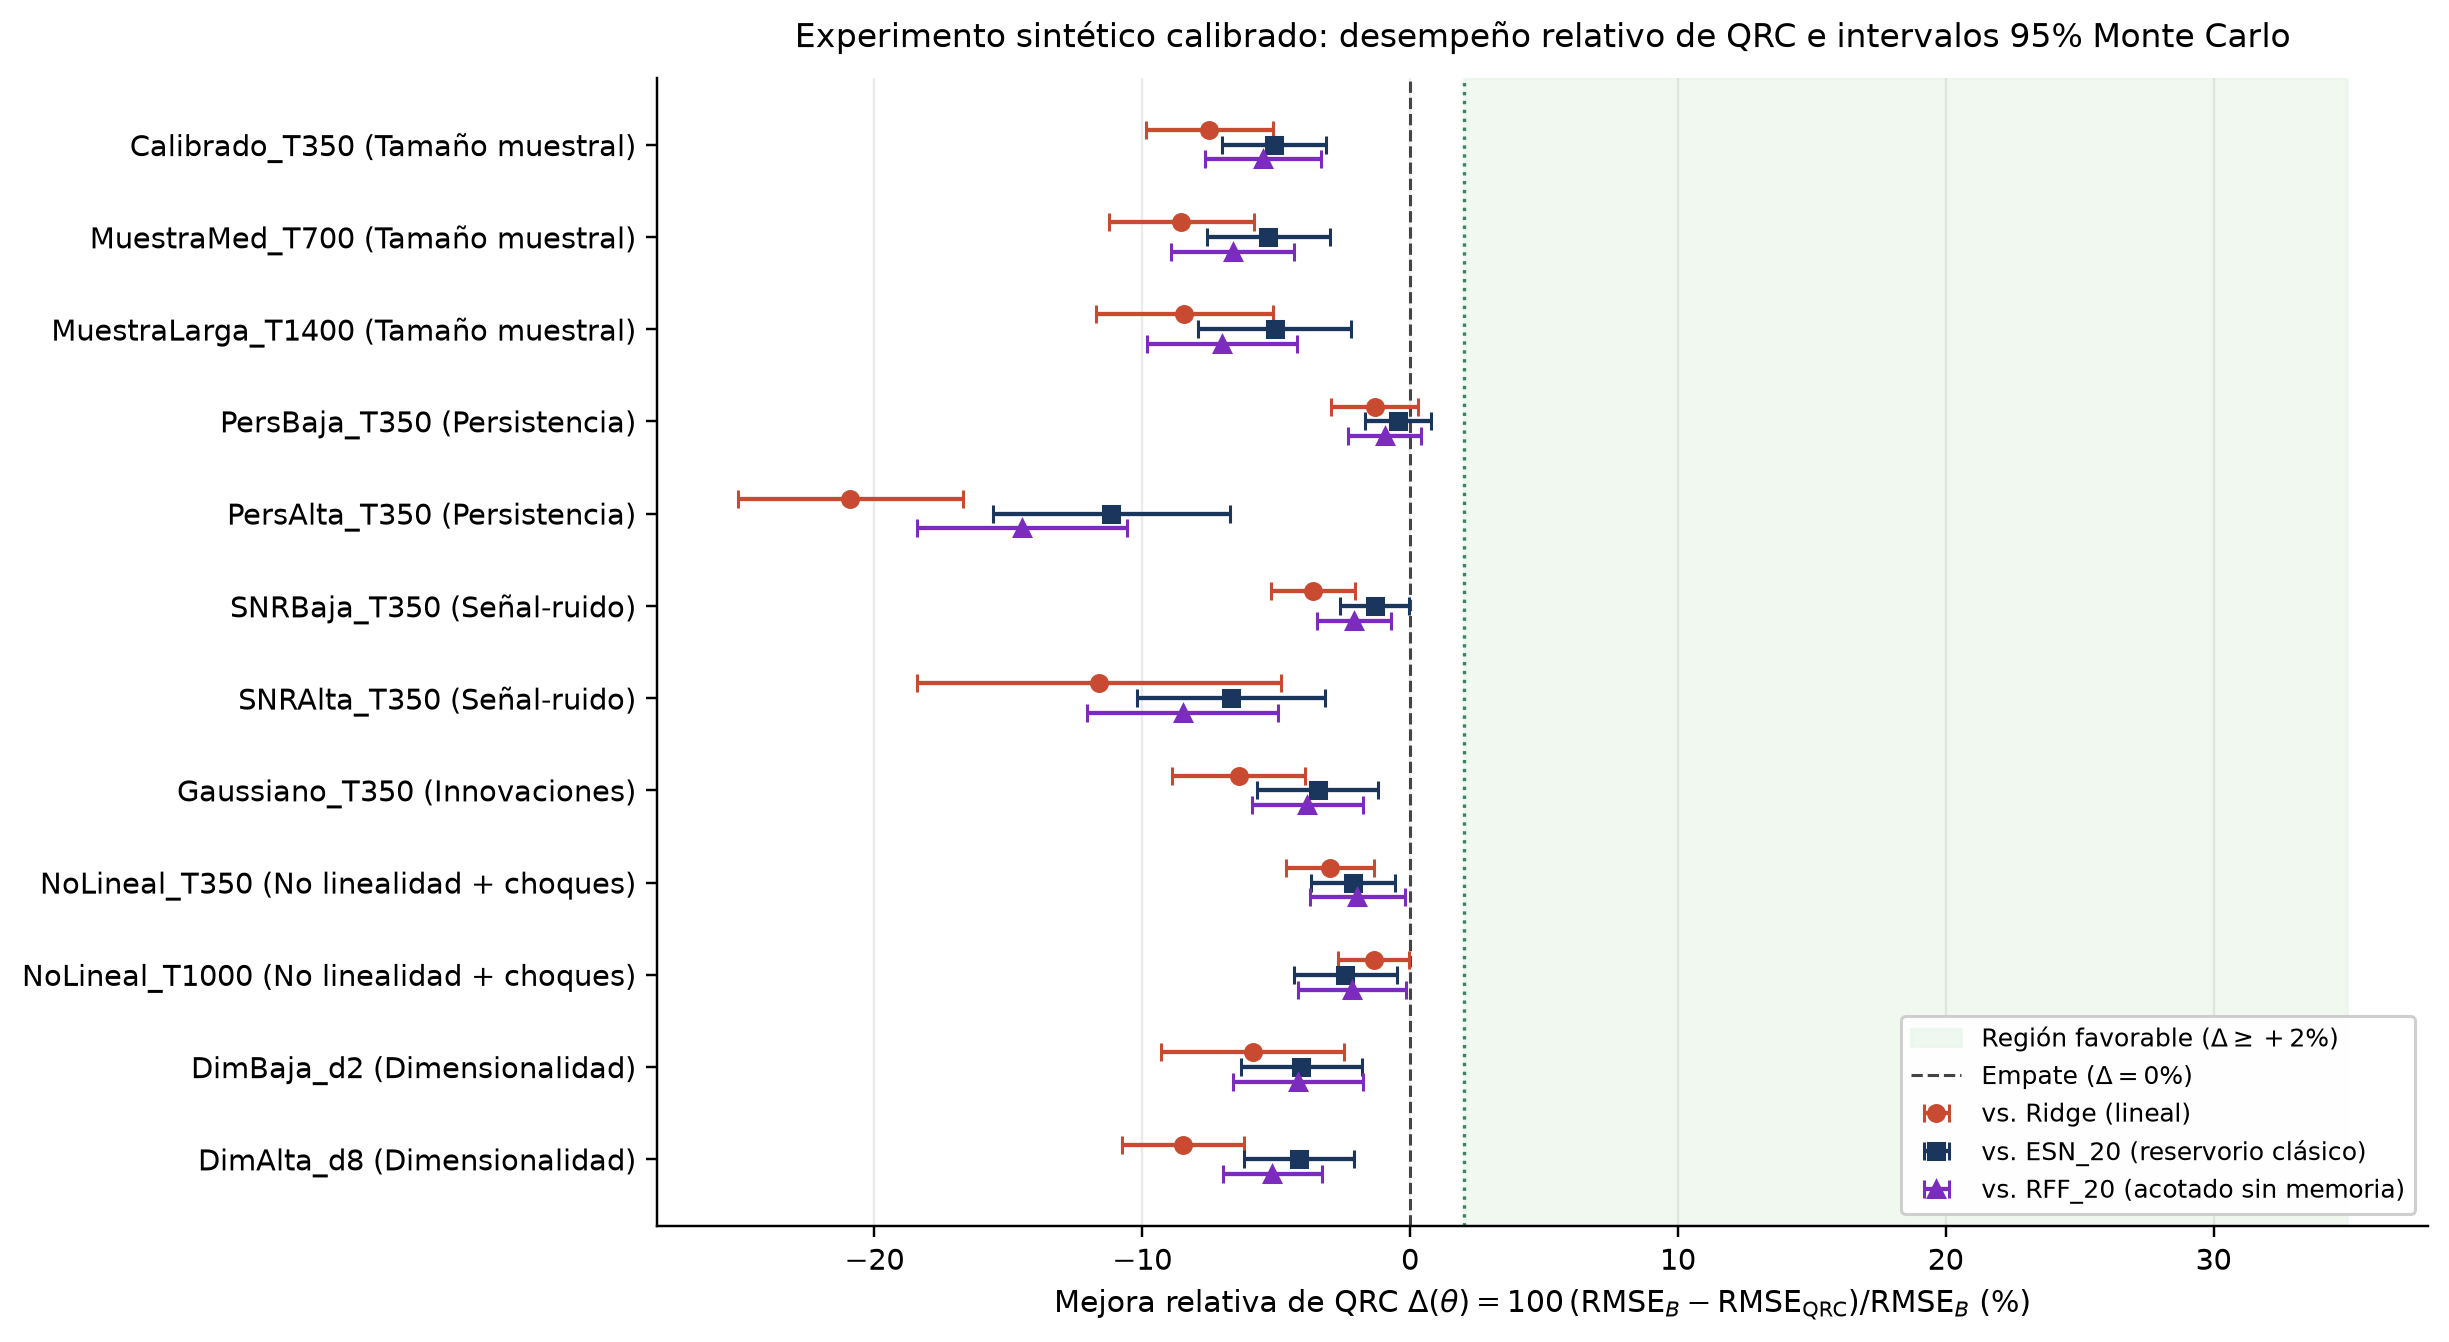
\includegraphics[width=0.94\textwidth]{figuras/etapa6_delta_escenarios.png}
  \apanota{Salidas de \codigo{output/etapa6\_sintetico/etapa6\_delta\_escenarios.png}. En los \(12\) escenarios evaluados la región favorable (\(\Delta \ge +2\%\) con intervalo positivo) permanece vacía (\(\mathcal{A}=\emptyset\)).}
\end{figure}

\begin{figure}[htbp]
  \caption{Efecto mínimo detectable (MDE al 80\% de potencia) y curvas bootstrap en \(n=250\)}
  \label{fig:etapa6_potencia}
  \centering
  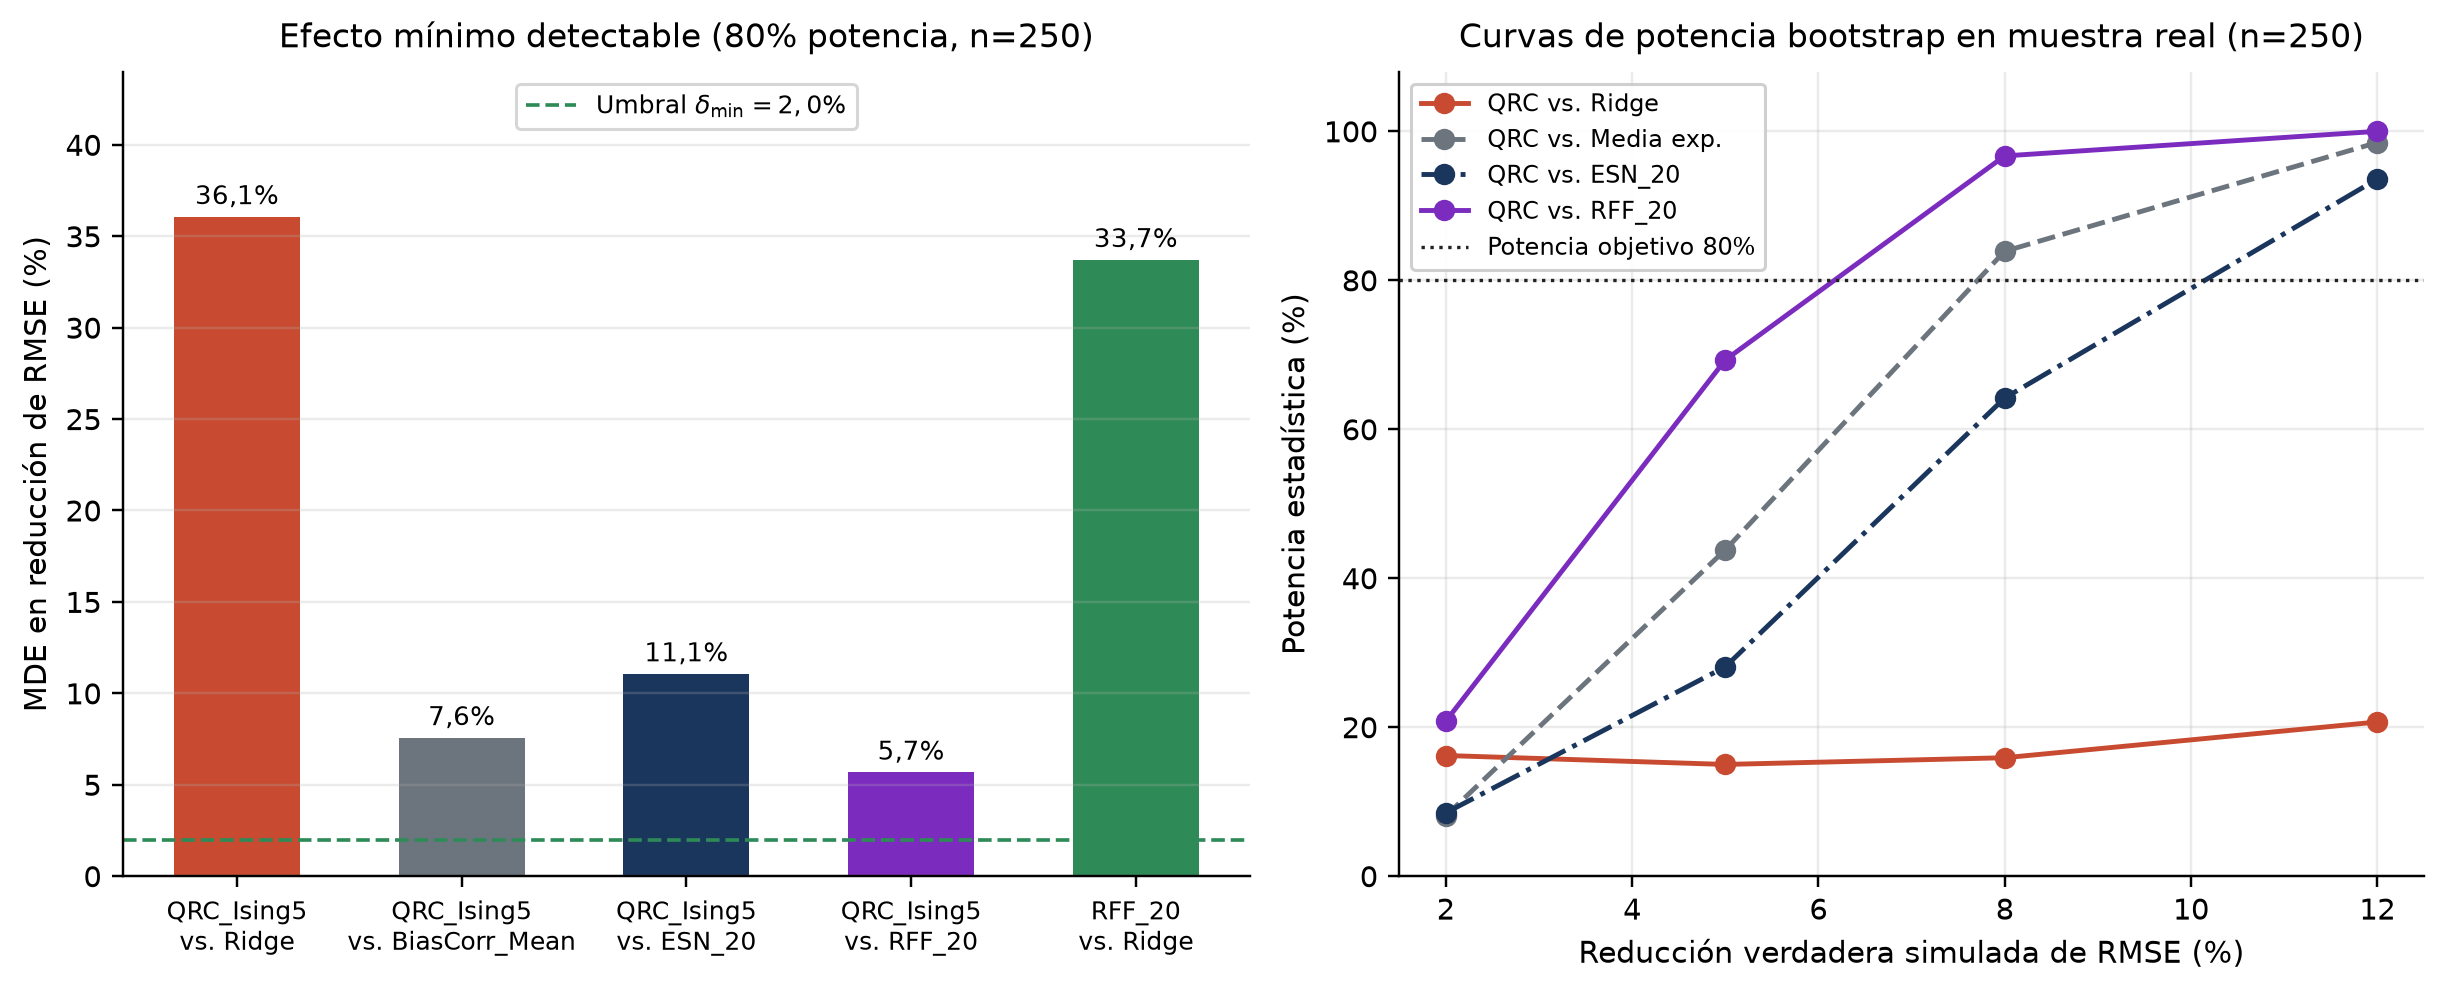
\includegraphics[width=0.94\textwidth]{figuras/etapa6_potencia_mde.png}
  \apanota{Salidas de \codigo{output/etapa6\_sintetico/etapa6\_potencia\_mde.png}. En la muestra peruana real, el MDE al 80\% es \(36{,}1\%\) frente a \codigo{Ridge}, \(11{,}1\%\) frente a \codigo{ESN\_20} y \(5{,}7\%\) frente a \codigo{RFF\_20}.}
\end{figure}

Las Figuras~\ref{fig:etapa6_delta} y~\ref{fig:etapa6_potencia} muestran que la región favorable sintética queda completamente vacía (\(\mathcal{A} = \emptyset\)) incluso con \(T=1\,400\) o dinámicas no lineales saturantes, donde \codigo{ESN\_20} y \codigo{RFF\_20} conservan una ventaja de \(\approx 2{,}2\%\)--\(2{,}4\%\) sobre QRC. Y en los datos reales (\(n=250\)), la potencia para detectar efectos modestos de \(2\%\) es apenas de \(8\%\)--\(21\%\). Con estos resultados verificados, el cierre programático de la Etapa~8 (\codigo{etapa8\_verificacion\_etapa7\_gate.json}) fija \texttt{etapa7\_activada = false}: por estricto rigor científico, se aplica la regla de paro preespecificada y no se monetiza una ganancia económica artificial atribuible a QRC.

Para reproducir o extender cualquier modelo nuevo respetando todas las garantías causales explicadas en este manual, el uso mínimo de \codigo{rtd\_eval\_utils.py} es el siguiente:

\begin{lstlisting}[language=Python, caption={Uso directo de las utilidades causales compartidas para nuevos modelos}]
from pathlib import Path
import scripts.rtd_eval_utils as u

# 1. Construir matriz causal con 20 predictores observables en v0(t)
df = u.build_realtime_feature_table(Path("output/analysis_output"))

# 2. Para cualquier origen t (p. ej. indice 100 = 2003m2), obtener entrenamiento sin fuga
tr_idx = u.get_causal_train_indices(df, eval_idx=100)
X_tr, X_te = u.fit_impute_and_scale(
    df.loc[tr_idx, u.FEATURE_COLS].to_numpy(),
    df.loc[[100], u.FEATURE_COLS].to_numpy()
)
\end{lstlisting}

\apabibliografia

\end{document}
